%        File: git-presentation.tex
%     Created: Wed Oct 17 12:00 PM 2012 NDT
%      Author: Siôn le Roux <sion@sionleroux.com>
%
% This work is licensed under a Creative Commons Attribution-ShareAlike 4.0
% International License. See the README.md file for more information.
%
% !TEX program = pdflatex

\documentclass{beamer}

\mode<presentation>
{
  \usetheme{Warsaw}
  \usecolortheme{seahorse}
  \usecolortheme{rose}
  \useinnertheme{rectangles}
  \setbeamercovered{transparent}
}

\usepackage[UKenglish]{babel}
\usepackage[utf8]{inputenc}
\usepackage{lmodern}
\usepackage[T1]{fontenc}
\usepackage{hyperref}
\usepackage{color}
\usepackage{graphicx}

\graphicspath{{screenshots/}}

\setlength\fboxsep{0.5pt}
\setlength\fboxrule{0.5pt}

\hypersetup{
  pdffitwindow=true,%
  pdftitle={Git \& Eclipse},%
  pdfauthor={Si\^on le Roux},%
  colorlinks=true,%
  pdfmenubar=false,%
  pdftoolbar=false,%
  bookmarks=false,%
  unicode=true,%
  linkcolor=black,%
  urlcolor=cyan
}

\title[Git \& Eclipse]{Collaborative Development}
\subtitle{Using git and Eclipse with the EGit and Mylyn plugins.}

\author{Si\^on~Le~Roux}

\date{\today}

\subject{Software Development}

%Show the ToC at the beginning of every section and sub-section
\AtBeginSection[]
{
  \begin{frame}{Overview}
    \tableofcontents[currentsection,currentsubsection]
  \end{frame}
}

\AtBeginSubsection[]
{
  \begin{frame}{Overview}
    \tableofcontents[currentsection,currentsubsection]
  \end{frame}
}

\begin{document}

\begin{frame}
  \titlepage
\end{frame}

\section{Introduction}
\begin{frame}[<+->]
  \frametitle{Introduction}
  \begin{itemize}
  \item Why are we doing this?
  \item Why git and Eclipse?
    \begin{itemize}
    \item \textbf{Git}: best VCS\footnote{\href{http://git-scm.com/about}{git-scm.com/about}}
    \item free project hosting on \textbf{GitHub}
    \item does \textbf{distributed} Version Control
    \item \textbf{Eclipse}: great Java IDE
    \item \textbf{plug-in based} architecture
    \end{itemize}
  \item Can we get a copy of this tutorial?\footnote{\href{http://sionleroux.com/files/git-presentation.pdf}{sionleroux.com/files/git-presentation.pdf}}
  \item What do we aim to achieve?
  \end{itemize}
\end{frame}

\section{Set-up}
\subsection{Git}
\begin{frame}[<+->]
  \frametitle{Installing Git}
  \begin{block}{GNU/Linux}
  Install git from your package manager. On Debian based systems, that's: \texttt{\# aptitude install git}
  \end{block}
  \begin{block}{Windows}
  \begin{enumerate}
    \item Download the \emph{Git for Windows} installer from \href{http://msysgit.github.com}{msysgit.github.com}
    \item Follow the installation instructions following the installer's recommended ``safe'' options.
  \end{enumerate}
  \end{block}\pause
  You can now type \textbf{\texttt{git}} at the command prompt, and access the Git GUI on Windows.
\end{frame}

\begin{frame}[<+->]
  \frametitle{Setting up Git}
  Follow instructions at \href{https://help.github.com/articles/set-up-git}{help.github.com/articles/set-up-git}

  In summary:\pause
  \begin{enumerate}
  \item If you don't have one, create an account at \href{http://github.com}{github.com}
  \item Generate a private-public ssh-keypair
  \item Add the public key on GitHub
  \item Set your name and e-mail in the global git config
  \end{enumerate}
  \begin{block}{Setting name and e-mail}
  \texttt{git config \--\--global user.name 'John Doe'}

  \texttt{git config \--\--global user.email 'johndoe@gmail.com'}
  \end{block}\pause
  You can learn git at \href{http://git-scm.com/book}{git-scm.com/book}
\end{frame}

\subsection{Eclipse}
\begin{frame}[<+->]
  \frametitle{Getting Eclipse}
  \begin{block}{GNU/Linux}
  Install eclipse from your package manager. On Debian based systems, that's: \texttt{\# aptitude install eclipse}
  \end{block}
  \begin{block}{Windows}
  \begin{enumerate}
    \item Download \emph{Eclipse Classic} from \href{http://www.eclipse.org/downloads/}{eclipse.org/downloads}
    \item Unzip the eclipse folder to \textit{Program Files}
    \item Create desktop and start menu shortcuts to \texttt{eclipse.exe}
  \end{enumerate}
  \end{block}
\end{frame}

\begin{frame}[<+->]
  \frametitle{Installing the Plug-Ins}
  \begin{itemize}
  \item Eclipse plug-ins can be installed from the marketplace:

    \texttt{Help > Eclipse Marketplace}
  \item The required plug-ins are:
    \begin{description}
    \item[EGit] for git support
    \item[Mylyn] for bugtracking and task management
    \item[Connector] GitHub Connector for Mylyn
    \end{description}
  \end{itemize}
  \begin{block}{Note}
    After restarting Eclipse you should be able to access the new Git and Task management perspectives:

  \begin{visibleenv}<6>
    
\includegraphics{perspectives}
  \end{visibleenv}
  \end{block}
\end{frame}

\section{Usage}

\subsection{EGit}
\begin{frame}
EGit provides the following context menu:

\fbox{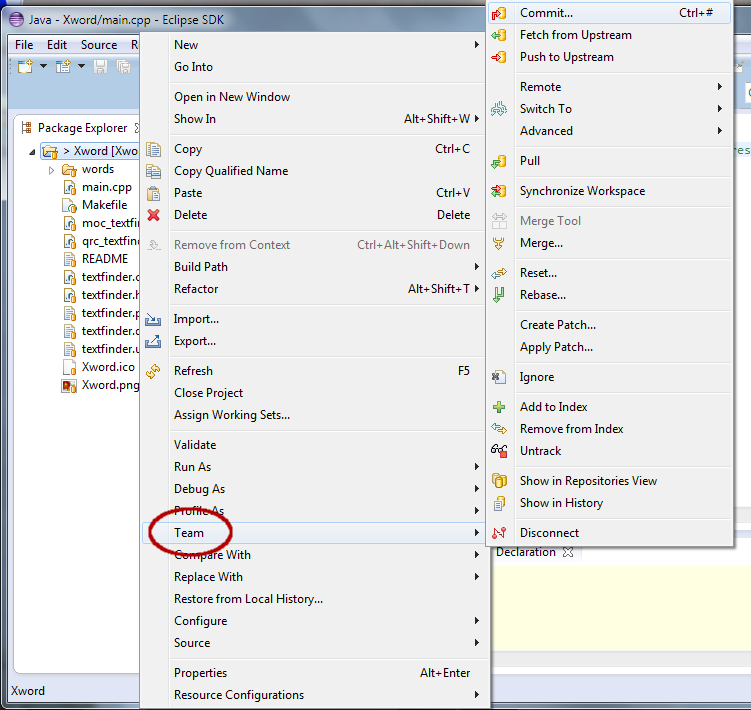
\includegraphics[width=0.7\textwidth]{team-context-menu}}
\end{frame}

\begin{frame}
  The following new perspective is also available:

  \fbox{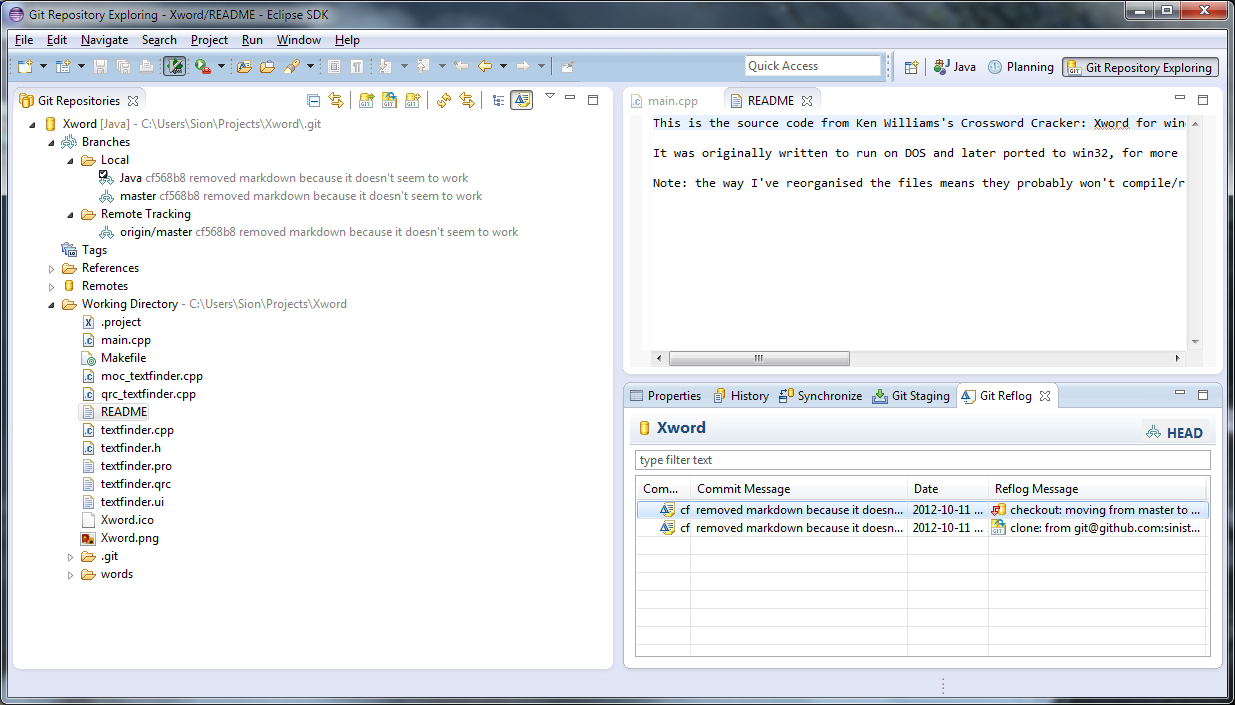
\includegraphics[width=\textwidth]{git-perspective}}
\end{frame}

\subsection{Mylyn}
\begin{frame}
  To use Mylyn you will first need to add a task repository:

  \fbox{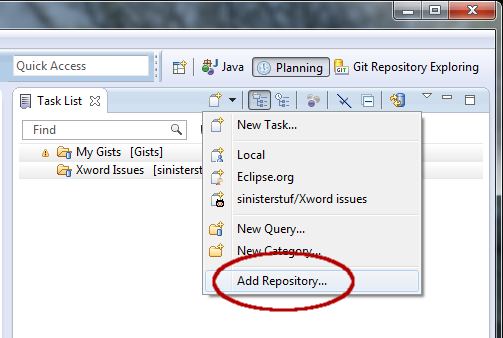
\includegraphics[width=\textwidth]{add-task-repo}}
\end{frame}

\begin{frame}
  You can then add issues which will be synced to GitHub's servers:

  \fbox{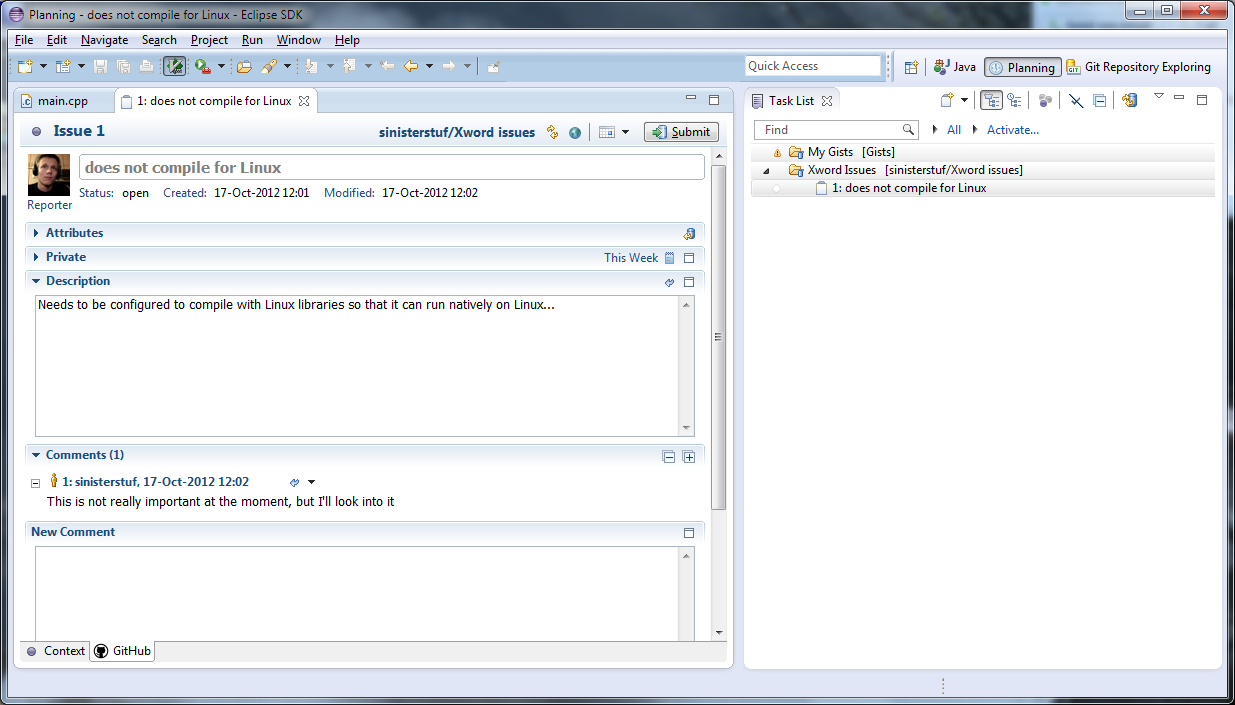
\includegraphics[width=\textwidth]{add-issue}}
\end{frame}

\subsection{GitHub}
\begin{frame}
  Now issues added in Eclipse will be added in the GitHub web interface:

  \fbox{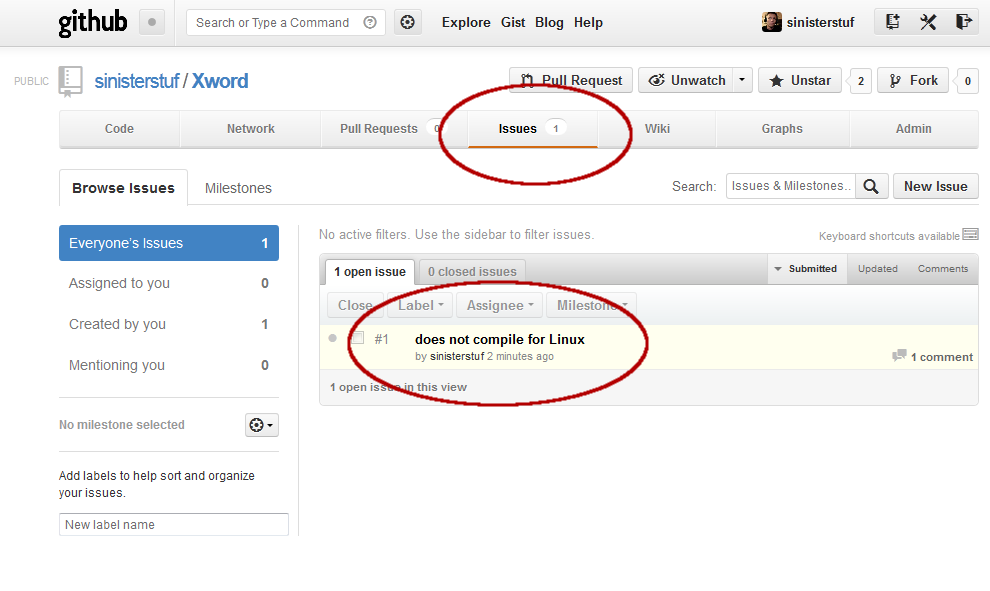
\includegraphics[width=0.95\textwidth]{github-issue-overview}}
\end{frame}

\begin{frame}
  We can also comment and manage issues on GitHub the same way as in Eclipse:

  \fbox{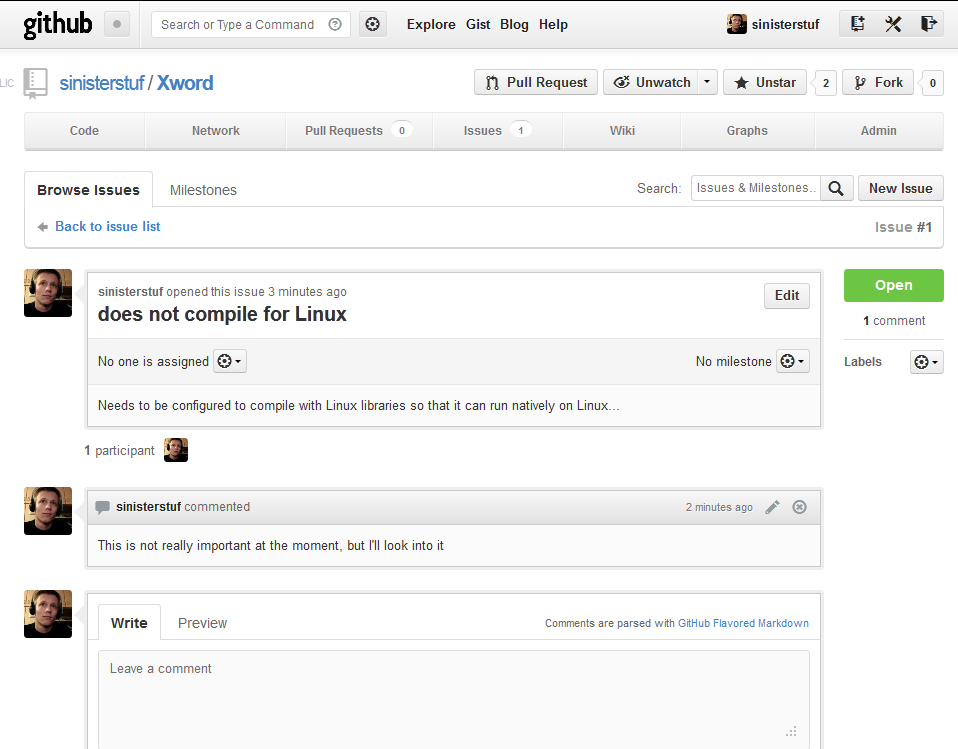
\includegraphics[width=0.7\textwidth]{github-issue-details}}
\end{frame}

\begin{frame}
  \begin{center}
  {\bfseries \Huge The End}
  \vspace{1cm}

  
\includegraphics[width=0.2\textwidth]{cc-by-sa.pdf}
  \end{center}
\end{frame}

\end{document}


